
% 中山大学科技类及IT类实验报告文档类(LaTeX模板)
\documentclass{sysucseexp}
\usepackage{fontspec,inconsolata,url}
\setmainfont{Times New Roman}
\setmonofont{Consolas}

% 载入需要的宏包
\input{settings/packages.tex}
% 进行必要的设置
\input{settings/format.tex}
% 专用术语宏命令进行必要的设置
\input{settings/terms.tex}

% 设置封面基本信息，\linebreak 前面不要有空格，
% 中文之间的空格无法消除
% 另，在\sysucseset中不可以出现空行
\sysucseset{
  college = {计算机学院},            % 学院名称
  projname = {计算复杂性理论实验},       % 实践课程名称
  title = {第一次编程作业},    % 实验报告题目
  stunoleader = {23336150},              % 组长学号
  authorleader = {刘昊},             % 组长姓名
  stunoone = {23336203},              % 组员1学号
  authorone = {任意嵘},             % 组员1姓名
  stunotwo = {23336193},              % 组员2学号
  authortwo = {彭怡萱},             % 组员2姓名
  major = {计算机科学与技术},          % 专业
  adviser = {冯剑琳},                   % 指导教师姓名
  startdate = {2026年3月23日},        % 实验起始日期
  enddate = {4月3日}        % 实验结束日期
}

\begin{document} %在document环境中撰写文档

%%%%%%%%%%%%%%%%%%%%%%%%%%%%%%%%%%%%%%%%
% 封面及目录，无需改动此处代码
\makecover
% 目录
\tableofcontents
\cleardoublepage
% 设置正文页眉页脚格式，并重新设置页码为1
\pagestyle{main} % 无页眉，页码在页脚居中
%%%%%%%%%%%%%%%%%%%%%%%%%%%%%%%%%%%%%%%%

% 排版正文内容
\section{实验目的与要求}

本次编程作业要求同学们以小组为单位，编写 Python 程序实现 \texttt{tm2.ppt} 中的图灵机编码、多带图灵机以及通用图灵机，并以两数加法图灵机 ADD 为测试用例进行测试。这三个部分的实现并不割裂，应当在同一个 Python 程序中组合完成整个工作流。

\textbf{项目已完成所有模块的实现}，包括图灵机编码、多带图灵机模拟器和通用图灵机模拟器。

具体的核心要求如下：
\begin{enumerate}
    \item \textbf{图灵机编码模块}
    \begin{itemize}
        \item 读取定义图灵机的 JSON 文件，并将其转换为二进制编码。
        \item 按照特定的规则，将元素映射为正整数：例如将图灵机的状态 $q_i$、符号 $X_j$ 和移动方向 $D_m$ 等映射之后，用 $0$ 的数量表示大小，元素间由 $1$ 隔开，最终转为由 $0$ 和 $1$ 构成的二进制字符串。
    \end{itemize}

    \item \textbf{多带图灵机模块}
    \begin{itemize}
        \item 实现一个多带图灵机模拟器，模拟实现多条磁带、多磁头的独立工作以及状态转移操作。
        \item \textbf{实时展示运行过程}：在多带图灵机的运行过程中，需要在屏幕上实时格式化打印出当前状态、各条磁带的内容（含边界分隔符等），以及各个磁头的位置。
        \item \textbf{执行模式控制}：程序应当支持两种展示模式：
        \begin{enumerate}
            \item \textbf{交互式}：图灵机每一步状态转移后，等待用户敲击空格键后继续下一步运行。
            \item \textbf{自动式}：图灵机每一步状态转移后，等待可配置的固定时间（例如 0.5 秒）后自动继续下一步运行。
        \end{enumerate}
    \end{itemize}

    \item \textbf{通用图灵机（UTM）模块}
    \begin{itemize}
        \item 基于多带图灵机的代码，实现通用图灵机模拟。
        \item 设定 UTM 初始状态下第一条磁带（Tape 1）包含完整输入 $M 111 w$。其中 $M$ 为通过编码模块获得的被模拟图灵机编码，$w$ 为该图灵机的输入字符串。
        \item 模拟时，Tape 2 专门用于存放模拟图灵机 $M$ 的纸带并标记 $M$ 的磁头位置；Tape 3 专门用于保存 $M$ 当前的状态。
        \item 为了简化实现，允许假定输入给通用图灵机的代码总是合法的，省略并跳过初始的合法性检查步骤（Step 1）。
        \item 除了多带图灵机常规的纸带实时打印外，还需在每次状态切换时根据 \texttt{tm2.ppt} 中的步骤，打印出\textbf{当前所处的运行阶段的完整说明文本}。
    \end{itemize}

    \item \textbf{用例测试}
    \begin{itemize}
        \item 构造 \texttt{tm more examples.pdf} 中两数加法图灵机 ADD 的 JSON 定义文件作为输入。
        \item 根据 JSON 里 \texttt{input} 字段（如 \texttt{["00", "000"]}，即分别代表输入 2 和 3 的一进制编码），执行 UTM 运转测试。
    \end{itemize}
\end{enumerate}

\section{模块设计思路}

\subsection{图灵机编码模块}
图灵机编码模块的主要功能是读取表示图灵机的 JSON 定义文件，解析出其中的状态及状态转移函数，将元素正确映射为独立的正整数，最终利用一进制（Unary）策略将图灵机的行为转换为纯粹的由 \texttt{0} 和 \texttt{1} 构成的二进制字符串。为保证编码过程的确定性与稳健性，具体设计思路展开如下：

\begin{enumerate}
    \item \textbf{JSON 解析、校验与归一化（Normalization）}：
    \begin{itemize}
        \item \textbf{容错校验}：程序读取 JSON 后，提取其中的字典结构。遍历每一个状态及其挂载的转移条件，严格校验是否存在 \texttt{write}, \texttt{move}, \texttt{nextState} 等核心字段。
        \item \textbf{字段归一化}：对于存在多种书写偏好的符号，进行底层归化以消除歧义。例如，将空白符的不同别名（如 \texttt{""}, \texttt{" "}, \texttt{"blank"} 等）统一转化为标准的单空格 \texttt{" "}；将移动方向（如大写的 \texttt{"L"}, \texttt{"Left"} 等）全部统一映射为内部标志 \texttt{left}, \texttt{right}、\texttt{stay} 以供直接调用。
    \end{itemize}

    \item \textbf{状态（States）的无碰撞 ID 映射}：
    \begin{itemize}
        \item \textbf{强制映射分配}：利用正则表达式 \texttt{\textasciicircum q([1-9]\textbackslash d*)\$} 提取符合标准命名的状态数字后缀，将其直接作为该图灵机状态的标号（例如，提取 \texttt{q1} 中的 $1$ 并分配极值给它）。为了防止 \texttt{q1} 的对应数字 1 被其他非标准状态误占，代码中会专门维护一个已用数字池（\texttt{used\_ids}）。
        \item \textbf{非标准状态的字典序填补}：如果存在其它命名规则的标志状态（如 \texttt{start}, \texttt{accept}等），将所有状态名称置于字典序下排序后，以递增遍历的方式为其寻找当前未被标记占用的最小正整数。通过两步解耦的设计彻底避免了标号碰撞。
    \end{itemize}

    \item \textbf{符号与方向的 ID 固定分配}：
    \begin{itemize}
        \item 根据实验规范对基础字符进行强绑定：数值 \texttt{0} 锁定对应 ID 1；数值 \texttt{1} 锁定对应 ID 2；空白符（\texttt{blank}）锁定为 ID 3。其余被图灵机使用的未知工作字符集合也将基于字典序从 4 开始向上顺序累加。
        \item 移动方向采用静态字典约束，按规定映射：\texttt{left}$\rightarrow 1$, \texttt{right}$\rightarrow 2$, \texttt{stay}$\rightarrow 3$。
    \end{itemize}

    \item \textbf{状态转移列表的稳健排序}：
    为了保证一台确定的图灵机会产生截然不变的编码字符串，必须在遍历所有状态转移生成代码之前对其做全排。模块采用了一个五维元组作为图灵机转移的排序 \texttt{KEY}：\texttt{((当前态ID), (读符号ID), (下状态ID), (写符号ID), (移动方向ID))}。

    \item \textbf{一进制拼接与组合连结}：
    排序完成后，针对五步数组中的每一个正整数编号 $N$，利用函数生成长度为 $N$ 的连续零串（例如 3 生成 \texttt{000}）。同一转移式中的五项动作内用单个 \texttt{1} 隔断；不同转移表达式之间最后连结时插入 \texttt{11} 成为全局统一编码。
\end{enumerate}

\subsection{多带图灵机模块}
多带图灵机模块实现了一个通用的多带图灵机模拟器，支持任意数量的磁带和磁头。核心设计思路如下：

\begin{enumerate}
    \item \textbf{磁带模型}：每条磁带使用无限长的字符列表表示，磁头位置用整数索引表示。磁带内容动态扩展，支持向左或向右无限延伸。
    
    \item \textbf{转移规则}：转移规则基于当前状态和所有磁带的当前读取符号，确定写入符号、移动方向和下一状态。使用元组表示多磁带的读取/写入/移动操作。
    
    \item \textbf{执行流程}：每步执行时，首先读取所有磁头的当前符号，查找匹配的转移规则，然后同时执行所有磁带的写入和移动操作，最后更新状态。
    
    \item \textbf{运行模式}：支持交互式（每步等待用户输入）和自动模式（固定时间间隔自动执行），便于观察和演示图灵机的运行过程。
    
    \item \textbf{状态管理}：维护当前状态、步数计数和停机标志。停机条件包括无匹配转移规则或进入接受状态。
\end{enumerate}

\subsection{通用图灵机模块}
通用图灵机（UTM）模块基于多带图灵机实现，按照 \texttt{tm2.ppt} 中的定义模拟任意单带图灵机。核心设计思路如下：

\begin{enumerate}
    \item \textbf{三带架构}：使用三条磁带实现UTM：
    \begin{itemize}
        \item Tape 1：存储被模拟图灵机的编码 $M$ 和输入 $w$，格式为 $M111w$
        \item Tape 2：模拟被模拟图灵机的磁带，使用一进制编码表示符号
        \item Tape 3：存储被模拟图灵机的当前状态，使用一进制编码
    \end{itemize}
    
    \item \textbf{编码解析}：从图灵机编码中解析转移规则。编码格式为一系列转移的二进制串，每个转移包含状态ID、符号ID、下一状态ID、写入符号ID和移动方向ID的一进制表示。
    
    \item \textbf{符号表示}：每个被模拟图灵机的符号用 $k$ 个UTM符号表示，其中 $k$ 是状态ID和符号ID的最大值，用于确保唯一性。
    
    \item \textbf{执行阶段}：按照 \texttt{tm2.ppt} 的步骤执行：
    \begin{itemize}
        \item Step 1：验证编码合法性（简化实现中跳过）
        \item Step 2：分析符号表示长度
        \item Step 3：初始化三条磁带
        \item 主循环：查找匹配转移并执行，直到停机或接受
    \end{itemize}
    
    \item \textbf{转移执行}：在Tape 2上修改符号表示，根据移动方向调整磁头位置，更新Tape 3上的状态编码。
    
    \item \textbf{接受判断}：当被模拟图灵机进入接受状态时，UTM也接受。
\end{enumerate}

\section{关键代码展示}

\subsection{图灵机编码：转移序列的确定性多键排序}
利用 Python \texttt{sorted} 内置方法与多重映射，保证编码输出无论 JSON 顺序如何都恒定一致：
\begin{lstlisting}[language=Python]
# src/modules/encoding.py (片段)
ordered_transitions = sorted(
    transitions,
    key=lambda transition: (
        state_ids[transition.current_state],
        symbol_ids[transition.read_symbol],
        state_ids[transition.next_state],
        symbol_ids[transition.write_symbol],
        DIRECTION_IDS[transition.move],
    ),
)
\end{lstlisting}

\subsection{图灵机编码：防冲突的状态 ID 映射逻辑}
优先预留 \texttt{qN} 的固有位值，后续按字典序填补空挡寻找正整数。
\begin{lstlisting}[language=Python]
def build_state_ids(transitions: List[Transition]) -> Dict[str, int]:
    state_names = { # 通过集合推导式去重合并起点与终点状态
        transition.current_state for transition in transitions
    } | {transition.next_state for transition in transitions}

    state_ids: Dict[str, int] = {}
    used_ids: Dict[int, str] = {}

    # 阶段1：严格提取规范化 qN 中的数字 N 进行挂载
    for state_name in sorted(state_names):
        match = STATE_NAME_PATTERN.fullmatch(state_name)
        if not match:
            continue
        state_id = int(match.group(1)) # 取出数字
        # 异常校验已省略
        state_ids[state_name] = state_id
        used_ids[state_id] = state_name

    # 阶段2：对剩余的一般化字符串补充映射
    next_available = 1
    for state_name in sorted(state_names):
        if state_name in state_ids:
            continue
        while next_available in used_ids: # 探查下一个空置数值
            next_available += 1 
        state_ids[state_name] = next_available
        used_ids[next_available] = state_name
        next_available += 1

    return state_ids
\end{lstlisting}

\subsection{图灵机编码：一进制翻译核心封装}
将单个转移元组格式化为一进制序列并将全集编码串联起来：
\begin{lstlisting}[language=Python]
def encode_transition(
    transition: Transition,
    state_ids: Dict[str, int],
    symbol_ids: Dict[str, int],
) -> str:
    # 逐项转换为 N 个 0 表示的等效一进制数组
    parts = [
        unary_encode(state_ids[transition.current_state]),
        unary_encode(symbol_ids[transition.read_symbol]),
        unary_encode(state_ids[transition.next_state]),
        unary_encode(symbol_ids[transition.write_symbol]),
        unary_encode(DIRECTION_IDS[transition.move]), # left:1, right:2
    ]
    return "1".join(parts) # 元素内部只用一个 1 作为隔离符

# 对全局数组应用并聚合
return EncodingResult(
    encoding="11".join(item.encoding for item in encoded_transitions), # 语句间夹杂 11 
    # ... 其他结构
)
\end{lstlisting}

\subsection{多带图灵机核心代码}


多带图灵机通过 \texttt{MultiTapeTM} 类实现，该类支持:
\begin{itemize}
    \item 多条磁带和多个磁头
    \item 状态转移
    \item 交互式和自动两种展示模式
\end{itemize}

类的核心属性包括：

\subsubsection{初始化多带图灵机}
\begin{itemize}
    \item \texttt{initial\_state}：初始状态
    \item \texttt{num\_tapes}：磁带数量
    \item \texttt{accept\_states}:接受状态集合，如果为None则停机状态即为接受
    \item \texttt{tapes}：磁带对象列表，每个磁带有独立的磁头位置和内容
    \item \texttt{transitions}：转移规则字典，键为 (当前状态, 读取符号元组)，值为转移对象
    \item \texttt{halted}：是否已停机
    \item \texttt{step\_count}：执行步数计数
\end{itemize}

\subsubsection{设置指定磁带的内容和磁头位置}
\begin{itemize}
    \item \texttt{tape\_index}:磁带索引（从0开始）
    \item \texttt{read\_symbols}:每条磁带读取的符号元组
    \item \texttt{write\_symbols}:每条磁带写入的符号元组
    \item \texttt{moves}:每条磁带的移动方向元组 ("left", "right", "stay")
    \item \texttt{next\_state}:下一状态
\end{itemize}

\subsubsection{转移规则}
\begin{itemize}
    \item \texttt{current\_state}:当前状态
    \item \texttt{content}: 磁带内容字符串
    \item \texttt{head\_position}:磁头初始位置（默认为0）
\end{itemize}


核心方法 \texttt{step()} 实现了单步执行逻辑：

\begin{enumerate}
    \item 检查是否已停机，如果是则返回 \texttt{False}
    \item 获取所有磁带当前磁头位置的符号，构成读取符号元组
    \item 根据当前状态和读取符号查找匹配的转移规则
    \item 如果找不到匹配规则，设置停机标志并返回 \texttt{False}
    \item 执行转移：对每个磁带写入新符号并移动磁头
    \item 更新当前状态和步数
    \item 检查是否进入接受状态，如果是则设置停机标志
    \item 返回 \texttt{True} 表示成功执行一步
\end{enumerate}

\begin{lstlisting}[language=Python]
class MultiTapeTM:
    """多带图灵机类"""
    
    def __init__(self, num_tapes: int, initial_state: str, accept_states: Optional[set] = None):
        self.num_tapes = num_tapes
        self.tapes: List[Tape] = [Tape() for _ in range(num_tapes)]
        self.current_state = initial_state
        self.initial_state = initial_state
        self.accept_states = accept_states or set()
        self.transitions: Dict[Tuple[str, Tuple[str, ...]], MultiTapeTransition] = {}
        self.halted = False
        self.step_count = 0
    
    def step(self) -> bool:
        """执行一步转移"""
        if self.halted:
            return False
        
        current_symbols = self.get_current_symbols()
        key = (self.current_state, current_symbols)
        
        if key not in self.transitions:
            self.halted = True
            return False
        
        transition = self.transitions[key]
        
        # 执行写入和移动
        for i, tape in enumerate(self.tapes):
            tape.write(transition.write_symbols[i])
            tape.move(transition.moves[i])
        
        self.current_state = transition.next_state
        self.step_count += 1
        
        if self.current_state in self.accept_states:
            self.halted = True
        
        return True
\end{lstlisting}

\subsection{通用图灵机核心代码}


通用图灵机通过 \texttt{UniversalTuringMachine} 类实现，该类基于多带图灵机模拟任意单带图灵机。

UTM使用三条磁带：
\begin{itemize}
    \item \texttt{Tape1}:存储 M111w（被模拟图灵机的编码和输入）
    \item \texttt{Tape2}:存储当前状态和读取符号
    \item \texttt{Tape3}:存储转移规则。向左：回退到前一个符号的开始位置；向右：继续读取下一个符号；停留：保持当前位置不变
\end{itemize}

核心的 \texttt{step()} 方法实现了UTM的单步执行逻辑：

\begin{enumerate}
    \item 检查UTM是否已停机，如果是则返回 \texttt{False}
    \item 从Tape2解码当前磁头位置的符号ID（通过读取连续的0数量）
    \item 设置阶段为"search\_move"，在被模拟图灵机的转移规则中查找匹配的转移
    \item 如果找不到匹配的转移，设置阶段为"no\_match"，停机并返回 \texttt{False}
    \item 设置阶段为"execute\_move"，执行转移操作：
    \begin{itemize}
        \item 在Tape2上清除并写入新的符号编码
        \item 根据移动方向调整Tape2磁头位置
        \item 更新Tape3上的状态编码
    \end{itemize}
    \item 增加步数计数
    \item 检查被模拟图灵机是否进入接受状态，如果是则设置阶段为"accept"，UTM接受并停机
    \item 返回 \texttt{True} 表示成功执行一步
\end{enumerate}

符号解码和转移执行：
\begin{itemize}
    \item \texttt{\_decode\_symbol\_from\_tape2()}：从Tape2读取连续0的数量来解码符号ID
    \item \texttt{\_find\_matching\_transition()}：在编码的转移规则中查找匹配的状态和符号
    \item \texttt{\_execute\_transition()}：执行具体的转移操作，包括符号写入和磁头移动
\end{itemize}

说明：
\begin{itemize}
    \item 磁头位置用"*"标记
    \item 模式默认为"interactive"(交互式)，若使用自动模式，设置mode == "auto"
\end{itemize}


\begin{lstlisting}[language=Python]
class UniversalTuringMachine:
    """通用图灵机类"""
    
    def step(self) -> bool:
        """执行一步UTM操作"""
        if self.state.halted:
            return False
        
        # 获取当前状态和符号
        current_symbol_id = self._decode_symbol_from_tape2()
        
        # 搜索匹配的转移
        self.state.stage = "search_move"
        transition = self._find_matching_transition(self.simulated_state_id, current_symbol_id)
        
        if transition is None:
            self.state.stage = "no_match"
            self.state.halted = True
            return False
        
        # 执行转移
        self.state.stage = "execute_move"
        self._execute_transition(transition)
        self.state.step_count += 1
        
        # 检查是否进入接受状态
        state_name = self._get_state_name_by_id(self.simulated_state_id)
        if state_name in self.accept_states:
            self.state.stage = "accept"
            self.state.accepted = True
            self.state.halted = True
        
        return True
\end{lstlisting}

\section{运行结果展示}

\subsection{图灵机编码模块测试}
运行交互式入口程序并选择对应功能模块：
\begin{lstlisting}[language=bash]
请选择功能:
1. 列出 test 目录下的共享 JSON 样例
2. 对选定样例执行图灵机编码
3. 运行多带图灵机模拟器
4. 运行通用图灵机模拟器
5. 退出程序
请输入编号: 2
请选择测试样例:
1. sample_tm.json (test/sample_tm.json)
请输入编号: 1
\end{lstlisting}
对应的输出结果如下，得到按照给定规则的一连串 \texttt{0} 与 \texttt{1} 的正确编码结果（如图 \ref{fig:encode_result} 所示）：

\begin{figure}[H]
    \centering
    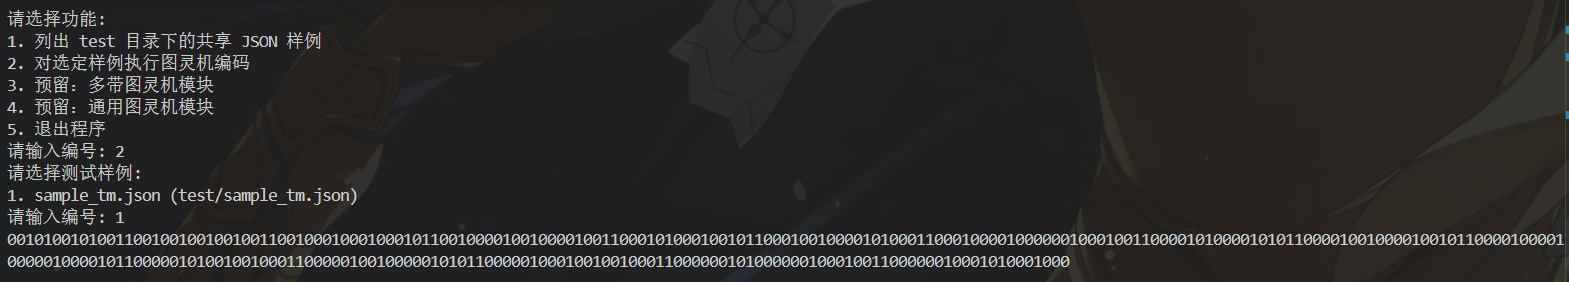
\includegraphics[width=0.9\textwidth]{figs/图灵机编码结果演示.png}
    \caption{图灵机编码模块交互与结果输出截屏}
    \label{fig:encode_result}
\end{figure}

\subsection{多带图灵机功能测试}

多带图灵机模拟器实现了对多带图灵机的完整模拟，支持交互式和自动运行模式。测试使用了一个简单的两带图灵机示例，该图灵机在Tape 1上读取输入字符串，在Tape 2上进行辅助计算，最终在7步后进入接受状态。

测试样例说明：
\begin{itemize}
    \item 磁带数量：2条
    \item 初始状态：q1
    \item 接受状态：halt
    \item Tape 1初始内容：0101（表示输入字符串）
    \item Tape 2初始内容：空（用"*"表示磁头位置），本次初始化 2 条磁带是为后续扩展做铺垫，保证代码框架的一致性
\end{itemize}

运行过程展示了每一步的状态变化、磁带内容和磁头位置的变化。图灵机通过多步转移最终将Tape 1的内容处理为0110，并在Tape 2上完成辅助计算，进入halt接受状态。

多带图灵机模拟器运行结果如下：
\begin{lstlisting}[language=bash]
============================================================
多带图灵机模拟器
============================================================
运行模式: interactive

==================================================
初始状态
==================================================
当前状态：q1
步数：0
Tape 1:      *0101
----------------------------------------
Tape 2:      *

按 Enter 键继续下一步...
==================================================
第 1 步
==================================================
当前状态：q1
步数：1
Tape 1:      0*101
----------------------------------------
Tape 2:      *

按 Enter 键继续下一步...
==================================================
第 2 步
==================================================
当前状态：q1
步数：2
Tape 1:      01*01
----------------------------------------
Tape 2:      *

按 Enter 键继续下一步...
==================================================
第 3 步
==================================================
当前状态：q1
步数：3
Tape 1:      010*1
----------------------------------------
Tape 2:      *

按 Enter 键继续下一步...
==================================================
第 4 步
==================================================
当前状态：q1
步数：4
Tape 1:      0101*
----------------------------------------
Tape 2:      *

按 Enter 键继续下一步...
==================================================
第 5 步
==================================================
当前状态：q2
步数：5
Tape 1:      010*1
----------------------------------------
Tape 2:      *

按 Enter 键继续下一步...
==================================================
第 6 步
==================================================
当前状态：q2
步数：6
Tape 1:      01*00
----------------------------------------
Tape 2:      *

按 Enter 键继续下一步...
==================================================
第 7 步
==================================================
当前状态：halt
步数：7
Tape 1:      0*110
----------------------------------------
Tape 2:      *

==================================================
结果：接受 (ACCEPTED)
总步数：7
==================================================
\end{lstlisting}

结合核心转移规则分析：
\begin{itemize}
    \item \texttt{规则1（q1 状态）}：磁头下为0/1（数字符号）→仅右移磁头，不修改符号，保持 q1 状态
    \item \texttt{规则2（q1→q2 的触发）}：1 状态下，磁头走到 Tape1末尾空白位（0101*后无符号，触发边界规则）→左移磁头，状态从 q1 切换为 q2
    \item \texttt{规则3（q2 状态）}：磁头下为1→写 0 覆盖，左移磁头，保持 q2 状态
    \item \texttt{规则4（q2→halt 的触发）}：磁头下为0（010*0）→写 1 覆盖，右移磁头，状态切换为 halt（接受态）
\end{itemize}

\subsection{通用图灵机功能测试}

通用图灵机（UTM）实现了对任意图灵机的模拟，通过三带架构来执行编码后的图灵机描述。测试使用了一个简单的单带图灵机编码，该图灵机将输入字符串"01"转换为"10"。

UTM工作原理：
\begin{itemize}
    \item Tape 0：存储被模拟图灵机的编码描述
    \item Tape 1：模拟被模拟图灵机的磁带
    \item Tape 2：存储UTM的内部状态和工作空间
\end{itemize}

测试过程展示了UTM如何逐步解析编码描述，执行相应的状态转移，并在有限步内完成计算。UTM通过读取Tape 0上的编码信息，在Tape 1上执行实际的图灵机计算，最终产生正确的输出结果。

通用图灵机模拟器运行结果如下（以两数加法图灵机为例）：
\begin{lstlisting}[language=bash]
============================================================
通用图灵机模拟器 (UTM)
============================================================
测试样例: add_tm.json
运行模式: interactive
最大步数: 10000

============================================================
UTM 初始化
============================================================
当前阶段说明：Step 2: The UTM examines M to see how many of its own tape squares it needs to represent one symbol of M.
符号表示长度：8 个UTM符号

当前阶段说明：Step 3: Initialize Tape 2 to represent the tape of M with input w, and initialize Tape 3 to hold the start state.

============================================================
初始状态
============================================================
============================================================
UTM 步数：0
被模拟图灵机状态ID：1
Tape1 (M111w):      *010101010011010010100100110100010010001001100101001010011001001001001001100100010001000101100010100001000101100010010000010101100010001000000100010110000101000010101100001001000010010110000100010000001000101100000101000001001011000001001000001010110000010001000010010110000001010000000100010011000000100100000001000100110000001000100000000100010001100000001010000000101001100000001001000000010010011000000010001000000001000100011100 000
----------------------------------------
Tape2 (模拟磁带):      *0101000101010
----------------------------------------
Tape3 (状态):      *0
当前阶段说明：Step 3: Initialize Tape 2 to represent the tape of M with input w, and initialize Tape 3 to hold the start state.
============================================================

按 Enter 键继续下一步...
============================================================
UTM 步数：1
被模拟图灵机状态ID：1
Tape1 (M111w):      *010101010011010010100100110100010010001001100101001010011001001001001001100100010001000101100010100001000101100010010000010101100010001000000100010110000101000010101100001001000010010110000100010000001000101100000101000001001011000001001000001010110000010001000010010110000001010000000100010011000000100100000001000100110000001000100000000100010001100000001010000000101001100000001001000000010010011000000010001000000001000100011100 000
----------------------------------------
Tape2 (模拟磁带):      01*01000101010
----------------------------------------
Tape3 (状态):      *0
当前阶段说明：If found, change the symbol and move the head marker on Tape 2 and change the State on Tape 3.
============================================================

按 Enter 键继续下一步...
============================================================
UTM 步数：2
被模拟图灵机状态ID：1
Tape1 (M111w):      *010101010011010010100100110100010010001001100101001010011001001001001001100100010001000101100010100001000101100010010000010101100010001000000100010110000101000010101100001001000010010110000100010000001000101100000101000001001011000001001000001010110000010001000010010110000001010000000100010011000000100100000001000100110000001000100000000100010001100000001010000000101001100000001001000000010010011000000010001000000001000100011100 000
----------------------------------------
Tape2 (模拟磁带):      01* 1000101010
----------------------------------------
Tape3 (状态):      *0
当前阶段说明：If found, change the symbol and move the head marker on Tape 2 and change the State on Tape 3.
============================================================

按 Enter 键继续下一步...
============================================================
UTM 步数：3
被模拟图灵机状态ID：2
Tape1 (M111w):      *010101010011010010100100110100010010001001100101001010011001001001001001100100010001000101100010100001000101100010010000010101100010001000000100010110000101000010101100001001000010010110000100010000001000101100000101000001001011000001001000001010110000010001000010010110000001010000000100010011000000100100000001000100110000001000100000000100010001100000001010000000101001100000001001000000010010011000000010001000000001000100011100 000
----------------------------------------
Tape2 (模拟磁带):      0001*000101010
----------------------------------------
Tape3 (状态):      *00
当前阶段说明：If found, change the symbol and move the head marker on Tape 2 and change the State on Tape 3.
============================================================

按 Enter 键继续下一步...
============================================================
UTM 步数：4
被模拟图灵机状态ID：3
Tape1 (M111w):      *010101010011010010100100110100010010001001100101001010011001001001001001100100010001000101100010100001000101100010010000010101100010001000000100010110000101000010101100001001000010010110000100010000001000101100000101000001001011000001001000001010110000010001000010010110000001010000000100010011000000100100000001000100110000001000100000000100010001100000001010000000101001100000001001000000010010011000000010001000000001000100011100 000
----------------------------------------
Tape2 (模拟磁带):      *0001   101010
----------------------------------------
Tape3 (状态):      *000
当前阶段说明：If found, change the symbol and move the head marker on Tape 2 and change the State on Tape 3.
============================================================

按 Enter 键继续下一步...
============================================================
UTM 步数：5
被模拟图灵机状态ID：6
Tape1 (M111w):      *010101010011010010100100110100010010001001100101001010011001001001001001100100010001000101100010100001000101100010010000010101100010001000000100010110000101000010101100001001000010010110000100010000001000101100000101000001001011000001001000001010110000010001000010010110000001010000000100010011000000100100000001000100110000001000100000000100010001100000001010000000101001100000001001000000010010011000000010001000000001000100011100 000
----------------------------------------
Tape2 (模拟磁带):      *0001   101010
----------------------------------------
Tape3 (状态):      *000000
当前阶段说明：If found, change the symbol and move the head marker on Tape 2 and change the State on Tape 3.
============================================================

按 Enter 键继续下一步...
============================================================
UTM 步数：6
被模拟图灵机状态ID：8
Tape1 (M111w):      *010101010011010010100100110100010010001001100101001010011001001001001001100100010001000101100010100001000101100010010000010101100010001000000100010110000101000010101100001001000010010110000100010000001000101100000101000001001011000001001000001010110000010001000010010110000001010000000100010011000000100100000001000100110000001000100000000100010001100000001010000000101001100000001001000000010010011000000010001000000001000100011100 000
----------------------------------------
Tape2 (模拟磁带):      000*1   101010
----------------------------------------  
Tape3 (状态):      *00000000
当前阶段说明：M accepts, the UTM also accepts.
----------------------------------------
Tape3 (状态):      *00000000
当前阶段说明：M accepts, the UTM also accepts.
============================================================

============================================================
运行结束
============================================================
当前阶段说明：M accepts, the UTM also accepts.
结果：接受 (ACCEPTED)
总步数：6
============================================================
\end{lstlisting}
\end{document}
